\section{Supplementary methods}

These sections provide more detailed descriptions of the mathematical
models and numerical approximations considered.

\subsection{Mathematical models and definitions}
\label{sec:more_maths}


\subsubsection{Notation}

In terms of geometrical domains, we consider the parenchyma
$\Omega_{\rm PAR} \subset \R^3$ and CSF spaces $\Omega_{\rm CSF}
\subset \R^3$ with $\Omega = \Omega_{\rm PAR} \cup \Omega_{\rm CSF}$
(see also \Cref{fig:intracranial_domains}). The coordinates in these
3D domains is given by $x$. The interface between the parenchyma and
CSF spaces is given by $\partial \Omega_{\rm PAR} \cap \partial
\Omega_{\rm CSF}$ and we separate it as two parts: the surface of the
lateral ventricles $\Gamma_{\rm LV}$ and the remaining pial interface
$\Gamma_{\rm pia}$ (thus $\partial \Omega_{\rm CSF} \bigcap \partial
\Omega_{\rm PAR} = \Gamma_{\rm LV} \cup \Gamma_{\rm pia}$). The
remaining, outer, boundary of $\Omega_{\rm CSF}$ is again separated
into two parts: $\Gamma_{\rm SSAS}$ represents the lower interface
towards the spinal subarachnoid space (SSAS), while $\Gamma_{\rm AM}$
is the outer interface towards the arachnoid and dura
membranes. $\Gamma_{\rm AM}$ is further subdivided into its lower and
upper parts: $\Gamma_{\rm AM-L}$ and $\Gamma_{\rm AM-U}$. The boundary
of the spinal cord is denoted by $\Gamma_{\rm{SC}}$ and given by
$\Gamma_{\rm{SC}} = \partial \Omega_{\rm PAR} \setminus \partial
\Omega_{\rm CSF}$.


In addition, we consider two sets of perivascular networks represented
as graphs: a periarterial network $\Lambda_a$ represented by the
(connected) centerlines $\Lambda^i_{(a)}$ of the arterial tree, and a
perivenous network $\Lambda_v$ corresponding to the centerlines
$\Lambda^i_{(v)}$ of the veins. Recall that we represent the vascular
domains as the union of cylindrical vessels of radius $R_1^i$
surrounding the centerlines $\Lambda^i$. Moreover, we consider the
surrounding perivascular spaces as the union of annular cylinders
$\Omega^i$ of inner radius $R_1^i$ and outer radius $R_2^i > R_1^i$
and thus of width $R_2^i - R_1^i$. We denote the outer lateral surface
of the periarterial and perivenous spaces by $\Gamma_a$ and $\Gamma_v$, respectively. We
omit the subscript $a$ or $v$ when referring to any such network,
vessel segment or perivascular outer surface. We assume that $\Gamma$
is parametrized by the coordinate $s$, and with a minor abuse of
notation, simply write $s \in \Lambda$ to represent the point ${\bm
  \lambda}(s)$ on $\Lambda$ corresponding to $s$.

\subsubsection{Solute transport and exchange in intracranial domains (3D) and perivascular networks (1D)}

In this section, we describe the mathematical
model~\eqref{eq:multi_transport}, the associated definitions,
interface and boundary conditions in further detail. We refer to the
main text for explicit parameter values and give the general, abstract
form here. Recall that we model a concentration field $c = c(x, t)$
for $x \in \Omega$, $t > 0$ defined in $\Omega_{\rm PAR}$ and
$\Omega_{\rm CSF}$ separately. In each of these domains, $c$ satisfies
\begin{equation}
  \partial_t (\phi c) - \nabla \cdot (D \nabla (\phi c) ) + \nabla \cdot (\bm u c ) + \xi (\overline{c} - \hat c ) \delta_\Gamma = f \quad \quad \mathrm{in} \quad \Omega_{\rm CSF}, \Omega_{\rm{PAR}}.
  \label{eq:3d_pde}
\end{equation}
In~\eqref{eq:3d_pde}, $\phi$ is the fluid volume fraction (also known as the porosity) defined in the parenchyma ($\phi \ll 1$ in $\Omega_{\rm PAR}$) and in the CSF spaces ($\phi = 1$ in $\Omega_{\rm CSF}$). In the parenchyma, $\phi$ represents the extracellular space volume fraction. Moreover, $D$ is the effective diffusion coefficient of the relevant solute in the respective media which takes different values over the CSF spaces and the parenchyma, depending on tortuosity~\cite{sykova2008diffusion} and dispersive effects; and $\bm u$ is a convective velocity field representing the flow of CSF in $\Omega_{\rm CSF}$ and the flow of ISF in $\Omega_{\rm PAR}$. $\xi$ models a transfer or exchange parameter between the 3D domain ($\Omega_{\rm PAR}$ or $\Omega_{\rm CSF}$) and the perivacular networks $\Lambda_a, \Lambda_v$. To summarize,
\[
\phi =  \begin{cases}
  1  & \mathrm{in} \;  \Omega_{\rm{CSF}} \\ 
  \phi_{\rm{PAR}} & \mathrm{in} \; \Omega_{\rm{PAR}} 
  \end{cases}, \; 
D = \begin{cases}
  D_{\rm{CSF}} & \mathrm{in} \;  \Omega_{\rm{CSF}} \\ 
  D_{\rm{PAR}} & \mathrm{in} \; \Omega_{\rm{PAR}} \end{cases}, \; 
  \quad \bm u  = \begin{cases}
  \bm{u}_{\rm{CSF}} & \mathrm{in} \; \Omega_{\rm{CSF}} \\ 
  \bm{u}_{\rm{PAR}} & \mathrm{in} \; \Omega_{\rm{PAR}} 
\end{cases}, \; 
\xi = \begin{cases}
  \xi_{\rm{CSF}} & \mathrm{if} |\Omega^i \cap \Omega_{\rm{CSF}}| \neq 0 \\
  \xi_{\rm{EF}} & \mathrm{if} |\Omega^i \cap \Omega_{\rm{PAR}}| \neq 0  
\end{cases} . 
\]
In the above, $\xi$ is defined segment-wise: for each centerline $\Lambda^i$ with surrounding PVS $\Omega^i$, $|\Omega^i \cap \Omega_{\rm{PAR}}|$ (resp. $|\Omega^i \cap \Omega_{\rm{CSF}}|$) is nonzero whenever $\Omega^i$ intersects $\Omega_{\rm{PAR}}$ (resp. $\Omega_{\rm{CSF}}$). If the surrounding PVS intersects both, then we set $\xi = \xi_{\rm EF}$  if $\Omega^i$ mainly ($80$ percent) intersects $\Omega_{\rm{PAR}}$ in which case the interaction with $\Omega_{\rm{CSF}}$ (resp. $\Omega_{\rm{PAR}}$) is ignored; otherwise, we set $\xi = \xi_{\rm CSF}$. 
 
\fixme{Also in~\eqref{eq:3d_pde}, the notation $\overline{c}$ denotes a lateral average of the concentration over the outer perivascular surfaces, defined for each centerline $\Lambda^i$ and each point $s \in \Lambda^i$ by}
\begin{equation}
  \overline{c}(s) = \frac{1}{P(s)} \int_{\partial \Theta(s)} c 
\end{equation}
\rami{where $\partial \Theta(s)$ is the outer boundary of the cross-section $\Theta(s)$ of the PVS $\Omega^i$ at $s$ and $P(s)$ is the area of $\Theta(s)$.} For both the periarterial and perivenous networks ($\Lambda_a, \Lambda_v$ with outer PVS boundaries $\Gamma_a, \Gamma_v$), the (Dirac delta) term $\delta_\Gamma$ is a distribution concentrated on the outer lateral surfaces of the PVSs. \discuss{More precisely, it is defined in terms of its action on any sufficiently smooth function $v : \Omega \rightarrow \R$ and for each $\Lambda^i \subseteq \Lambda$ with PVS $\Omega^i$ and outer lateral surface $\Gamma^i = \partial \Omega^i_2$ by}
\begin{equation}
  %\xi (\overline{c} - \hat c ) \delta_\Gamma (v) = \int_{\Lambda} P \xi ( \overline{c} - \hat c ) \overline{v} .
  \delta_\Gamma (v) = \int_{\Gamma} v = \sum_{i} \int_{\Gamma^i} v = \sum_i \int_{\Lambda^i} P \, \overline{v} = \int_{\Lambda} P  \, \overline{v} .
\end{equation}
where $P = P(s)$ is defined as the perimeter of each cross-section $\Theta(s)$ for $s \in \Lambda^i$. 

\mer{MER: Stopped here. Feel free to check the above. I thought the overline was defined as the cross-section perimeter average and not the cross-section average. This is more compatible with the definition of $\delta_{\Gamma}$ as well.}

We refer to the reference~\cite{masri2023modelling} for a complete model derivation and analysis.

The above is supplemented with the following boundary conditions. 
\begin{alignat}{2}
(D \nabla (\phi c) - \bm u c ) \cdot \bm{n}_{\rm SAS} &= g_{\mathrm{influx}} &&  \quad  \mathrm{on} \quad \spinal  \\ 
% (-D \nabla (\phi c) + \bm u c ) \cdot \bm{n}_{\spinal} &= 0 &&  \quad  \mathrm{on} \quad \spinal^{\mathrm{out}}  \\ 
(-D \nabla (\phi c) + \bm u c ) \cdot \bm{n}_{\rm skull} & =   \beta c  &&  \quad  \mathrm{on} \quad \Gamma_{\rm skull^{u}}  \\ 
(-D \nabla (\phi c) + \bm u c ) \cdot \bm{n}_{\rm skull} & =   0  &&  \quad  \mathrm{on} \quad \Gamma_{\rm skull^{l}}  \\ 
(-D \nabla (\phi c_{\rm{PAR}}) + \bm u_{\rm{PAR}} c_{\rm{PAR} }) \cdot \bm{n}_{\rm{Pia}} &= - (-D \nabla  c_{\rm{CSF}} + \bm u_{\rm CSF} c_{\rm CSF} ) \cdot \bm{n}_{\rm{Pia}} &&  \quad  \mathrm{on} \quad \pia \cup \Gamma_{\mathrm{LV}}  \\ 
(-D \nabla (\phi c_{\rm{PAR}}) + \bm u_{\rm{PAR}} c_{\rm{PAR} }) \cdot \bm{n}_{\rm{Pia}} & = \beta_{\rm{pia}} (c_{\rm PAR} - c_{\mathrm{CSF}}) &&  \quad  \mathrm{on} \quad \pia \cup \Gamma_{\mathrm{LV}}   .  
\end{alignat} 

%When convenient, we also denote $c|_{\Omega_{\rm PAR}} = c_{\rm PAR}$
%and $c|_{\Omega_{\rm CSF}} = c_{\rm CSF}$.


In the above, note that $\bm u \cdot \bm n  \neq 0$ on $\Gamma_{\rm LV} \cup \Gamma_{\rm skull^u}$ and $\bm u \cdot \bm n = 0$ on $\Gamma_{\rm SSAS} \cup \Gamma_{\rm skull^l} \cup \Gamma_{\rm Pia}$. 

At bifurcation nodes in $\Gamma_a, \Gamma_v$, we impose flux conservation and continuity of the concentration $\hat c$. We refer to \eqref{eq:flux_conservation} in \Cref{sec:details_numerical_method} for more details. For the perivascular network, the boundary nodes are collected into $\partial \Lambda$. We assume no tracer outflow on all boundary nodes and prescribe a homogeneous Neumann condition: 
\begin{equation}
    \hat D A \partial_s (\phi \hat c) - A \hat u \hat c  = 0 \quad \mathrm{on} \quad \partial \Lambda. 
\end{equation}


Further, $P$ and $A$ are the perimeter and area of the PVS which can vary along the centerline network, respectively.  Finally, we remark that $\hat u$ takes different values on each $\Lambda_i$.  Both $\Omega$ and $\Lambda$ are fixed in time and we assume constant-in- time radii (despite varying radii to drive peristaltic flow, see \cref{sec:sup:peristalsis}). Finally, we note that the model assumes that there is no interaction between the inner perivascular boundary and the blood vessel. 


\paragraph*{Interface conditions}
On the interface $\Gamma_{\mathrm{pia}}$ between the CSF and brain, we prescribe the following condition modeling a semi--permeable pial interface 
\begin{alignat}{2}
(-D \nabla (\phi c_{\rm{PAR}}) + \bm u_{\rm{PAR}} c_{\rm{PAR} }) \cdot \bm{n}_{\rm{PAR}} &= - (- D \nabla c_{\rm{CSF}} + \bm u_{\rm{CSF}} c_{\rm{CSF}} ) \cdot \bm{n}_{\rm{PAR}} &&  \quad  \mathrm{on} \quad \pia \cup \Gamma_{\mathrm{LV}} ,  \\  
(-D \nabla ( c_{\rm{PAR}}) + \bm u_{\rm{PAR}} c_{\rm{PAR} }) \cdot \bm{n}_{\rm{PAR}} & = \beta_{\rm{pia}} (c_{\rm PAR} - c_{\mathrm{CSF}}) &&  \quad  \mathrm{on} \quad  \pia \cup \Gamma_{\mathrm{LV}} .  
\end{alignat} 
Here, $\beta_{\mathrm{pia}}$ is a permeability constant between the brain and the CSF:

\paragraph*{Boundary conditions}
On $\Gamma_{\mathrm{skull}}$, the interface towards the dura and skull (\Cref{fig:concept}), we consider a constant uptake (or efflux) rate, represented by the boundary condition 
\begin{alignat}{2}
(- D \nabla ( c_{\mathrm{CSF}}) + \bm u_{\mathrm{CSF}} c_{\mathrm{CSF}}) \cdot \bm{n}   & = \beta c_{\mathrm{CSF}}  && \quad \mathrm{on} \quad \Gamma_{\mathrm{skull}^{\rm u}},\\ 
(-D \nabla c_{\rm CSF} + \bm u c_{\rm CSF}) \cdot \bm{n} & =  0   &&  \quad  \mathrm{on} \quad \Gamma_{\rm skull^{l}} , 
\end{alignat}
where $\beta$ represents a molecular outflow resistance. Here, we take $\beta = 10^{-4} \,\, \mathrm{mm}^2/\mathrm{s}$\cite{hornkjol2022csf}.


\subsubsection{Incompressible Stokes flow of CSF in the SAS and ventricular system}

We consider non-zero convection in the CSF space $u_{\rm CSF} \not = 0$ in \eqref{eq:multi_transport_3d} resulting from steady state CSF production.  Recall that $\Omega_{\mathrm{CSF}}$ represents the CSF space and that $\Gamma_{\mathrm{skull^{u/l}}}$ and $\Gamma_{\mathrm{pia}}$, $\Gamma_{\mathrm{LV}}$ represent the boundaries facing the upper and lower parts of the dura, the pia and the lateral ventricles, respectively.  Assuming CSF production in the choroid plexus located at the lateral ventricle wall, we solve the  steady state Stokes equations for the velocity and the pressure $(\bm u_{\mathrm{CSF}}, p_{\mathrm{CSF}})$ in the CSF domain: 
\begin{subequations}
    \begin{alignat}{2}
 - \mu \Delta \bm u_{\mathrm{CSF}} + \nabla p_{\rm{CSF}} & =  0 \quad && \mathrm{in} \,\,  \Omega_{\rm CSF}, \label{eq:momnetum_equation}  \\ 
 \nabla \cdot  \bm u_{\mathrm{CSF}} & = 0 \quad && \mathrm{in} \,\,   \Omega_{\rm CSF}, \label{eq:divergence_equation}  \\ 
\mu \nabla \bm u_{\mathrm{CSF}} \cdot \bm{n} -  p \bm n  &  = -R_0 ( \bm u \cdot \bm n ) \bm n\,\,   && \mathrm{on}  \label{eq:efflux_condition} \,\, \Gamma_{\mathrm{skull^u}}, \\ 
\bm u_{\mathrm{CSF}} & = 0 && \mathrm{on} \,\, \Gamma_{\rm{pia}} \cup \Gamma_{\mathrm{skull^l}} \Gamma_{\rm{SSAS}}  \\
\bm u_{\mathrm{CSF}} \cdot \bm n & = \frac{1}{ |\Gamma_{\rm LV}|}  u_{\rm in}, \quad \bm u \cdot \bm \tau = 0 \quad && \mathrm{on} \,\, \Gamma_{\rm{LV}} .  
\end{alignat}
\end{subequations}
Here, $\bm n$ denotes the unit outward normal to the boundary, $\mu$ is the CSF viscosity, and $\bm u_{\rm in}$ is the steady CSF flow across the lateral ventricle wall, see \Cref{tab:pvs:parameters}.
Condition \eqref{eq:efflux_condition} models an efflux site with positive resistance $R_0 \geq 0$. The Stokes system is solved with the finite element software $FEniCS$, stored and then subsequently read for all the relevant solute transport simulations. See Figure~\ref{fig:csf_flow_cardiac} for a streamline visualization of the obtained velocity profile and \Cref{sec:details_numerical_method} for details on the numerical algorithm employed.

We do not explicitly model convection within the brain parenchyma $\Omega_{\rm PAR}$, and thus set ${\bm u} = {\bm u}_{\rm PAR} = 0$ there. 

\subsubsection*{Dispersion in the CSF spaces}

In addition, CSF pulsates in the SAS and ventricular system with each
cardiac and respiratory cycle.


Taking the large spatial differences of pulsatile CSF flow into account, we compute the local diffusion enhancement factor $R$ in the CSF-filled space $\Omega_{\rm CSF}$ by combining a computational model of cardiac induced CSF flow with theoretical estimates for shear-augmented (Taylor) dispersion \cite{taylor1953dispersion, watson1983diffusion}.

Sharp et al \cite{keith2019dispersion} estimated the enhancement of diffusion in the spinal subarachnoid space due to dispersive effects to average 5.8 times that of purely molecular diffusion with a theoretical maximum of $10^6$. 

Similar to the case of CSF flow driven by production introduced in section \ref{sec:csf_fluid_vel}, we employ a Stokes flow model to predict CSF velocities at peak arterial dilation. In particular, we enforce a uniformly distributed inflow of $10$\,ml/s and $2$\,ml/s across the outer skull ($\Gamma_{\rm skull}$) and lateral ventricular surfaces ($\Gamma_{\rm LV}$) respectively, mimicking the effect of reduced CSF volume due to blood inflow. We prescribe a no-slip boundary condition on the pial surface $\Gamma_{\rm Pia}$ and zero-traction on the spinal boundary $\Gamma_{\rm SSAS}$, making the spinal compartment the only outflow route of CSF. Thus, we compute the cardiac-driven flow field by augmenting the Stokes flow model (eq. \ref{eq:momnetum_equation} and \ref{eq:divergence_equation}) with the following boundary conditions:

\begin{equation}\label{eq:cardiac_flow_bcs}
    \bm u = 0 \text{ on } \Gamma_{\rm Pia}; \quad 
    \mu \nabla \bm u \cdot \bm n - p \bm n = 0 \text{ on } \Gamma_{\rm SSAS}; \quad 
    \bm u = \frac{0.31 \cdot \bm n}{|\Gamma_{\rm LV}|} \,\text{ml/s} \text{ on } \Gamma_{\rm LV}; \quad
    \bm u = \frac{8 \cdot \bm n}{|\Gamma_{\rm skull}|} \,\text{ml/s} \text{ on } \Gamma_{\rm skull}.
\end{equation}

The obtained pressure field only account for viscous forces, albeit cardiac induced CSF flow is known to be unsteady and substantially impacted by transient inertial forces. Assuming an oscillatory flow with the heartbeat frequency $\omega = 2 \pi$, a mean gap width of the CSF-filled spaces of $2h=3$\,mm and CSF density $\rho=10^3\,\text{kg/m}^3$, the Womersley number $\alpha$ becomes $\alpha^2 = \frac{h^2 \omega \rho}{\mu} = 20.2$, which is unsteady. Based on theoretical considerations on the ratio of oscillatory flow to steady flow impedances in a tube, we account for inertial forces in the pulsatile flow by upscaling the computed viscous pressure field by a factor of $1 + \alpha^2 / 8$ (see \cite{van1998cardiovascular}, chapter. 4.3).

Further assuming unsteady dispersion, we follow Sharp et al \cite{keith2019dispersion} and calculate the enhancement factor $R$ from the non-dimensionalized pressure gradient $dP=\frac{|\nabla p|}{\omega \mu / h}$ as $R\approx dP^2 / \alpha^3$. Combining the computed pressure gradient with this scaling law yields a pointwise approximation of the dispersion factor. Finally, we account for the non-local nature of the dispersion mechanism by applying a smoothing technique to obtain a spatially varying, but locally averaged diffusion enhancement factor $R$ (see the visualization in \cref{fig:visualize_R} and \cref{sec:dispersion_details} for additional details).


\subsubsection{Perivascular fluid flow induced by pressure gradients}

The production of CSF in the choroid plexus generates a small, but consistent pressure gradient within the intracranial space. To compute the resulting CSF flow within the PVS, we solve 1D Darcy equations in the PVS network. The unknowns are the averaged PVS velocity, $u_{\rm pvs} = \langle u_{v,s} \rangle$, and the cross-section pressure $p_{\rm pvs} $ (assumed to be constant in each cross-section). The system is given by  \cite{daversin2022geometrically, gjerde2024directional} 
\begin{alignat}{2}
A \,  u_{\rm pvs}   + \frac{\kappa}{\mu} \, A \, \partial_{s} p_{\rm pvs} & = 0, &&  \quad \rm in  \,\, \Lambda  \\ 
-\partial_s (A \, u_{\rm pvs}) & = f, && \quad \rm in  \,\, \Lambda .  
\end{alignat} 
In the above, $A$ is the area of the PVS, $\mu$ is the dynamic viscosity, and $\kappa$ is derived from the assumption of Poiseuille
flow in the annular cross-section of the PVS \cite{daversin2022geometrically,tithof2022network}: 
\begin{equation}
\kappa = \frac18 \left( R_2^2 + R_1^2 - \frac{1}{\ln(R_2/R_1)} (R_2^2- R_1^2) \right). 
\end{equation}
On bifurcations, conservation of fluxes is enforced weakly and continuity of the pressure is enforced strongly (in the choice of the finite element spaces). 

Since the pressure gradient the caused by the steady production-driven CSF flow (see \cref{sec:csf_fluid_vel}), we impose the precomputed fluid pressure $p_{\rm CSF}$ on the networks root nodes:

\begin{equation}
    p_{\rm PVS} = p_{\rm CSF} \quad \text{ on } \Lambda^{\rm out}
\end{equation}

In case that the root does not lie within the CSF-space but the parenchyma, the CSF pressure is not yet computed. For that reason, we apply a simple extension technique to map the CSF pressure field into $\Omega_{\rm PAR}$. In particular, we solve a Laplace equation on $\Omega_{\rm PAR}$ with the CSF pressure on the Pial membrane ($\Gamma_{\rm Pia}$) as a boundary condition.

\subsection{Numerical Method}
\label{sec:details_numerical_method}
Here we provide details on the numerical method used to solve the coupled system. We are given a mesh $\mathcal{T}_h $, consisting of elements denoted by $E$, of $\Omega= \brain \cup \sas$.  The collection of all interior facets to $\Omega_{\rm PAR}$ (resp.  to $\Omega_{\mathrm{CSF}}$) is  denoted by $\mathcal{F}_{h,b}$ (resp. $\mathcal{F}_{h,c}$).  The union of all interior facets $\mathcal{F}_i = \mathcal{F}_{h,b} \cup \mathcal{F}_{h,c}$. Facets lying on the pial interface are denoted by $\mathcal{F}_{\pia}$, on the skull by $\mathcal{F}_{\skull}$, and on the spinal canal by $\mathcal{F}_{\spinal}$. Note that $\mathcal{F}_i \cap \mathcal{F}_{\pia} = \emptyset $. The union of all the facets is denoted by $\mathcal{F}_h$. The restriction of $\mathcal{T}_h $ to $\Omega_{\mathrm{CSF}}$ is denoted by $\mathcal{E}_{h}$. 
\subsubsection{CSF Flow}
We recall the system of equations that we approximate. Find $(\bm u, p)$ such that 
\begin{subequations}
    \begin{alignat}{2}
 - \mu \Delta \bm u + \nabla p & =  \bm 0 \quad && \mathrm{in} \,\,  \Omega_{\rm CSF}, \label{eq:momnetum_equation}  \\ 
 \nabla \cdot  \bm u & = 0 \quad && \mathrm{in} \,\,   \Omega_{\rm CSF}, \label{eq:divergence_equation}  \\ 
\mu \nabla \bm u \cdot \bm{n} -  p \bm n  &  = -R_0 ( \bm u \cdot \bm n ) \bm n, \,\,  \quad \bm u \cdot \bm \tau = 0 \quad  && \mathrm{on}  \label{eq:efflux_condition} \,\, \Gamma_{\mathrm{skull^u}}, \\ 
\bm u & = 0 && \mathrm{on} \,\, \Gamma_{\rm{pia}} \cup \Gamma_{\mathrm{skull^l}} \cup \Gamma_{\rm{SSAS}} \\
\bm u \cdot  \bm n   =  \frac{1}{|\Gamma_{\mathrm{LV}}|} u_{\mathrm{in}}  , & \; \; \bm u \cdot \bm \tau  = 0  && \mathrm{on} \;  \Gamma_{\mathrm{LV}},
\end{alignat}
\end{subequations}
We follow \cite{hong2016robust} and approximate the velocity field $u$ and the pressure $p$ with the following finite element spaces. 
\begin{align}
\bm V_h  & = \{ \bm v  \in H(\mathrm{div}; \Omega_{\mathrm{CSF}}): \; \bm v \vert_{E} \in \mathbb{BDM}^2 (E),  \; E \in \mathcal{E}_h; \;  \bm v \cdot \bm n = 0 \text{ on } \Gamma_{\rm{pia}} \cup \Gamma_{\mathrm{skull^l}} \cup \Gamma_{\rm{SSAS}}, \;\; \bm v \cdot \bm n = \frac{1}{|\Gamma_{\mathrm{LV}}|} u_{\mathrm{in}} \text{ on } \Gamma_{\mathrm{LV}} \} \\ 
S_h  & = \{q \in L^2(\Omega):  \;  q \vert_E \in \mathbb{P}^1(E),  \; E \in \mathcal{E}_h \}. 
\end{align}
Here, $H(\mathrm{div};\Omega)$ is the space of $L^2$ vector fields with $L^2$ divergence,  $\mathbb{BDM}^2$ is the Brezzi-Douglas--Marini element \cite{brezzi1987mixed} of order 2, and  $\bm n$ (resp. $\bm \tau$) is the unit outward normal (resp. tangent) vector.  
Given any vector $\bm v$, the normal and tangential components on each facet  are denoted by 
\[ 
\bm v_n = (\bm v \cdot \bm n)\bm n , \quad \bm v_t = (\bm v - \bm v_n). 
\]
Since $V_h \subset H(\mathrm{div}, \Omega_{\rm{CSF}})$, then $[\bm v_n] = 0 $ on $\mathcal{F}_{h,c}$. Continuity in the tangential component is enforced weakly via interior penalization. For notational simplicity, denote by $\mathcal{F}_{\Gamma}$ the facets lying on $\Gamma_{\rm{pia}} \cup \Gamma_{\mathrm{skull}} \cup \Gamma_{\rm{SSAS}} \cup \Gamma_{\mathrm{LV}}$. Define the form 
\begin{multline}
\mathcal{A}_h (\bm u, \bm v) = \sum_{E \in \mathcal{E}_h} \int_{E} \mu \nabla u : \nabla v - \sum_{
F \in \mathcal{F}_{h,c} \cup \mathcal{F}_{\Gamma} 
} \int_{F} \mu \{\nabla u\}\cdot \bm n_F \cdot [\bm v_t] 
\\ - \sum_{
F \in \mathcal{F}_{h,c} \cup \mathcal{F}_{\Gamma} 
} \int_{F} \mu \{\nabla v\}\cdot \bm n_F \cdot [\bm u_t]
+ \sum_{
F \in \mathcal{F}_{h,c} \cup \mathcal{F}_{\Gamma} 
} \frac{\sigma \mu}{h} \int_{F} [\bm u_t ] \cdot [\bm v_t].   
\end{multline}
We set $\sigma =20$. The discretization for the CSF flow, is then to find $(\bm u_h, p_h) \in \bm V_h \times S_h$ such  that 
\begin{align}
\mathcal{A}_h(u_h, v_h)  + \sum_{F \in \mathcal{F}_{\Gamma_{\mathrm{skull}}}} \int_{F} R_0 (\bm u_h \cdot \bm n) (\bm v_h \cdot \bm n) - \int_{\Omega} \nabla \cdot \bm v_h \, p_h  & = 0, \quad \forall \bm v_h \in \bm V_h   \\ 
(\nabla \cdot \bm u_h , q_h ) & = 0, \quad \forall q_h \in S_h.
\end{align}
\subsubsection{PVS flow} 


Recall that we compute pressure-driven flow within the PVS by solving a 1D Darcy equations in the PVS network. The unknowns are the averaged PVS velocity, $u_{\rm pvs} = \langle u_{v,s} \rangle$, and the cross-section pressure $p_{\rm pvs} $ (assumed to be constant in each cross-section). The system is given by  \cite{daversin2022geometrically, 
gjerde2024directional} 

\begin{alignat}{2}
A \,  u_{\rm pvs}   + \frac{\kappa}{\mu} \, A \, \partial_{s} p_{\rm pvs} & = 0, &&  \quad \rm in  \,\, \Lambda  \\ 
-\partial_s (A \, u_{\rm pvs}) & = f, && \quad \rm in  \,\, \Lambda .  
\end{alignat} 

where $A$ is the area of the PVS, $\mu$ is the dynamic viscosity, and $\kappa$ is derived from the assumption of Poiseuille flow in the annular cross-section of the PVS  \cite{daversin2022geometrically,tithof2022network}: 
\begin{equation}
\kappa = \frac18 \left( R_2^2 + R_1^2 - \frac{1}{\ln(R_2/R_1)} (R_2^2- R_1^2) \right). 
\end{equation}

As boundary conditions, we impose the precomputed fluid pressure $p_{\rm CSF}$ on the networks root nodes:

\begin{equation}
    p_{\rm PVS} = p_{\rm CSF} \quad \text{ on } \Lambda^{\rm out}
\end{equation}

In case that the root does not lie within the CSF-space but the parenchyma, the CSF pressure is not yet computed. For that reason, we apply a simple extension technique to map the CSF pressure field into $\Omega_{\rm PAR}$.
In particular, we solve the Laplace equation
\begin{equation}
    - \Delta p = 0; \quad p = p_{\rm CSF} \text{ on } \Gamma_{\rm Pia}
\end{equation}
to obtain the extension of $p_{\rm CSF}$ onto $\Omega_{\rm PAR}$.

To enforce conservation of flux and continuity of pressure on bifurcation points, we approximate the velocity with a piecewise discontinuous polynomials and the pressure with continuous piecewise polynomials, respectively. The finite element spaces thus are:

\begin{align}
   V_h^{\rm PVS} = \{v_h \in L^2(\Lambda): v_h \vert_{\Lambda_i} \in
   \mathbb{P}^{k -1}(\Lambda_i)\} \text{ and }
   Q_h^{\rm PVS} = \{ q_h \in C^0(\Lambda),  q_h \vert_{\Lambda^i} \in \mathbb{P}^k(\Lambda_i), q_h \vert_{\Gamma_{\rm Pia}} = p_{\rm CSF} \}
\end{align}

The weak form reads: Find $(u_{\rm PVS}, p_{\rm PVS}) \in V_h^{\rm PVS} \times Q_h^{\rm PVS}$ such that

\begin{align}
(A u_{\rm PVS}, v) + \left(v, \frac{A \kappa}{\mu} \partial_s p_{\rm PVS}  \right) &= 0 \quad \forall v \in V_h^{\rm PVS} \\
(A u_{\rm PVS} , \partial_s q ) &= 0 \quad  \forall q \in  Q_h^{\rm PVS}
\end{align}

where $\tau$ is the tangent vector of the network. Here we employ the lowest order discretization and set $k=1$. For discussion of stability of the discrete model we refer to \cite{gjerde2024directional}. 

\subsubsection{Solute transport}
For the 3D concentration, we use broken polynomial spaces and interior penalty discontinuous Galerkin (DG) methods with upwinding in order to capture the sharp boundary layers.  For DG, we utilize the discrete space 
\begin{equation}
V_h^k = \{v_h \in L^2(\Omega): \;  v_h \vert_E \in \mathbb{P}^k(E), \; E \in \mathcal{T}_h\}.
\end{equation}
To discretize the diffusion term, we utilize symmetric weighted interior penalty dG bilinear forms. We refer to \cite{ern2009discontinuous} and \cite[Section 4.5.2.3]{di2011mathematical} for details on this method.  We define 
\begin{multline}
a_h (c_h, v_h) = \sum_{E \in \mathcal{T}_h } \int_{E} D \nabla (\phi c_h) \cdot \nabla v_h + \sum_{F \in \mathcal{F}_i} \eta \frac{\gamma_{D,F}}{h_F} \int_{F} [c_h][v_h] 
- \sum_{F \in \mathcal{F}_i} \int_{F} \left( \{D \phi \nabla c_h \}_w \cdot \bm n_F [v_h]  + \{D \phi\nabla v_h \}_w \cdot \bm n_F [c_h] \right).
 \nonumber
 \end{multline}
In the above, for $F\in \mathcal{F}_h^i$ with a normal $n_F$ pointing from $E_F^1$ to $E_F^2$,  the jump is given by $[v_h] = v_h{}_{\vert_{E_F^1}} - v_h{}_{\vert_{E_{F}^2}}$, and the weighed average is defined as follows.
\begin{equation}
\{v_h\}_{w} = \frac{ \kappa_{\vert_{E_F^2}}}{\kappa_{\vert_{E_F^1}}+ \kappa_{\vert_{E_F^2}}} v_h{}_{\vert_{E_{F}^1}} + \frac{\kappa_{\vert_{E_F^1}}}{\kappa_{ \vert_{E_F^1}}+ \kappa_{\vert_{E_F^2}}} v_h{}_{\vert_{E_{F}^2}}, \quad \text{where} \quad \kappa = D \phi.  
\end{equation}
The parameter $\gamma_{D,F}$ is the harmonic mean of the diffusion coefficient given by 
$$
\gamma_{D,F} = \frac{ \kappa_{\vert_{E_F^1}}\kappa_{\vert_{E_F^2}}}{\kappa_{\vert_{E_F^1}}+ \kappa_{\vert_{E_F^2}}},
$$
and $\eta$ is a user specified penalty to be determined later. 

For the convection term, we use upwinding, see \cite[Section 2.3.1]{di2011mathematical} and the references therein. Define 
\begin{equation*}
a_h^{\mathrm{up}}(c_h, v_h) =- \sum_{E\in\mathcal{T}_h } \int_E \bm{u} c_h \nabla v_h  + \sum_{F \in \mathcal{F}_i } \int_F \{ \bm u  c_h\} \cdot \bm{n}_F [v_h]  + \sum_{F \in \mathcal{F}_i} \int_F \frac{|\bm u \cdot \bm n_F |}{2} [c_h ] [v_h ] 
\end{equation*}
The discrete formulation for \eqref{eq:3d_pde} then reads 
\begin{multline}
\int_{\Omega}\frac{1}{\tau} (\phi c_h^n - \phi c_h^{n-1}) v_h + a_h(c_h^n, v_h) + a_h^{\mathrm{up}}(c_h^n,v_h) + \int_{\Gamma_{\mathrm{pia}} } \beta_{\mathrm{pia}}[c_h^n][v_h]  \\ + \int_{\Gamma_{\rm skull^u}} \beta c_h^n v_h +  \int_{\Lambda} \xi  P (\overline{c_h^n} - \hat c_h^n) \overline{v_h}  = \int_{\Omega} f^n v_h + \int_{\spinal} \gin v_h , \quad \forall v_h \in V_h^k.
\end{multline}
For the 1D concentration $\hat c$, we recall that $\hat c = \hat c_i $ on each segment of the network $\Lambda^i$.  We enforce continuity of the concentration on the bifurcation points and conservation of fluxes. We let $\mathcal{V}$ denote the set of all vertices in $\Lambda$ and $ 
\mathcal{E}(\mathsf{v})$ denote the set of segments sharing a vertex $\mathsf{v}$.  For a given edge $\Lambda^i= (\mathsf{v}_\mathrm{in}^i, \mathsf{v}_{\mathrm{out}}^{i})$, we define the function $n_i: \mathcal{V} \rightarrow \{-1,0,1\}$ with $$
n_i(\mathsf{v}_{\mathrm{in}}^i) = 1 , \,\, n _i (\mathsf{v}_{\mathrm{out}}^i) = -1 \,\, \mathrm{and} \,\,\, n_i(\mathsf{v}) = 0, \quad \forall \mathsf{v} \in 
\mathcal{V} \,  \backslash \,  \{ \mathsf{v}_{\mathrm{in}}^\mathsf e,\mathsf{v}_{\mathrm{out}}^\mathsf e \}.  
$$
The collection of bifurcation points is denoted by $\mathcal{B} = \{ \mathsf{v} \in \mathcal{V}, \,\,  \mathrm{card}(\mathcal{E}(\mathsf{v})) \geq  3\}$. For any $\mathsf{v} \in \mathcal{B}$, we have 
\begin{equation}
\sum_{ i \in \mathcal{E}(\mathsf{v})} (\hat D A_i \phi \partial_s \hat{u}_i(\mathsf{v})  -  A_i \hat u_i(\mathsf{v}) \hat c_i(\mathsf{v})) n_i(\mathsf{v}) = 0  \label{eq:flux_conservation}
\end{equation}
For approximating the solution of the 1D equations in the network, we use the space 
\[ \hat V_h = \{ v_h \in C^0(\Lambda), 
\; v_h \vert_{\Lambda^i} \in V_h(\Lambda^i)
\}, 
\]
where $V_h(\Lambda^i)$ is the space of continuous polynomials of degree $1$ on each $\Lambda^i$, 

\subsection{Cardiac Dispersion Factor Estimation}\label{sec:dispersion_details}

To compute a spatially varying estimate of the diffusion enhancement factor $R$, we consider the Stokes flow problem (\cref{eq:momnetum_equation} and \cref{eq:divergence_equation}) equipped with the boundary conditions \cref{eq:cardiac_flow_bcs} describing cardiac induced CSF flow at peak arterial pulsation. We use the numerical method described in \cref{sec:details_numerical_method} to solve the Stokes system and compute the non-dimensionalized local pressure difference $dP=\frac{|\nabla p| \rho}{\omega \mu / h}$ pointwise. Here, $\mu$ is the CSF viscosity, $\omega = 2 \pi$ is the oscillatory heart beat frequency, $2h=3$\,mm the assumed gap width and $\rho=10^3\,\text{kg/m}^3$ the density of the CSF.

In addition, we account for inertial forces in the pulsatile flow by upscaling the obtained pressure gradient by a factor of $1 + \alpha^2 / 8$ (see \cite{van1998cardiovascular}, chapter. 4.3), where $\alpha^2 = \frac{h^2 \omega \rho}{\mu} = 20.2$ is the square of the Womersley number for an oscillatory flow.

Finally, we smooth the resulting field by solving a Helmholtz problem with $dP^2$ as the right-hand side

\begin{equation}
- 10^{-4} \Delta R + R = dP^2 \quad \text{ on } \Omega_{\rm CSF} \qquad \text{ and } \quad \nabla R \cdot \bm n = 0 \quad \text{ on } \partial \Omega_{\rm CSF}
\end{equation}

to obtain the locally averaged, spatially varying diffusion enhancement factor $R$.

\subsection{Estimating net perivascular flow induced by peristaltic waves}
\label{sec:sup:peristalsis}

We use the theoretical framework introduced by Gjerde et al.~\cite{gjerde2023directional} to compute an analytic estimate of the time-averaged (or \emph{net}) flow rates $\langle Q'_i \rangle$ (mm$^3$/s) induced by peristaltic pumping in a perivascular network$\Lambda = \cup_i \Lambda_i$. The motion of the (inner) vascular wall is described by a periodic traveling (peristaltic) wave of relative amplitude $\varepsilon$, wave length $\lambda$ (mm) and frequency $f$, acting normal to the wall. By definition, the wave number is $k = 2 \pi/\lambda$ and the angular frequency is $\omega = 2 \pi f$. Each PVS segment $\Lambda_i$ has length $L_i$ with wave-relative length $\ell_i = k L$, baseline inner radius $r_{o_i}'$, fixed outer radius $r_{e_i}'$, and outer-to-inner ratio $\beta_i = r_{e_i}'/r_{o_i}'$ (see also \Cref{tab:pvs:parameters}). These geometric parameters and the assumption of annular cylindrical PVS segments yield hydraulic resistances $\mathcal{R}_{o, i}$ and additional characteristic parameters, see \cite{gjerde2023directional} for the complete definitions and schematics. Since the analytical estimate is derived under the assumption that $k L \approx \mathcal{O} 1)$~\cite{gjerde2023directional} and has been verified against numerical simulations for $k L$ of the order $10^{-1}-10^2$~\cite[Table I]{gjerde2023directional}, we consider it applicable for the wave lengths and vascular network data considered here in which $k L$ ranges from \mer{$X$ to $Y$.}

\begin{table}
  \small
  \begin{tabular}{llrc}
    \toprule
    Parameter & Description & Value(s)  & Ref.\\ 
    \midrule
    Relative PVS size $\beta$ & $\beta = \beta_i = r_{e_i} / r_{o_i}$ & 2 & $\approx$\cite{eide2024functional} \\
    Wave frequency $f$ & Traveling wave frequency of vascular motion & $0.1-1.0$ Hz & \discuss{\cite{gjerde2023directional}} \\
    Wave length $\lambda$ & Traveling wave length of vascular motion & $20-2000$ mm & \discuss{\cite{broggini2024long, gjerde2023directional}} \\
    Wave amplitude & Relative amplitude of inner wall motion & $1-10\%$ & \discuss{\cite{gjerde2023directional}} \\
    Vascular radii $\{r_{o_i}\}$ & Vascular network radii data (avg $\pm$ std, $\min$, $\max$) & $X$, $X$, $X$  mm & \cite{hodneland2019new} \\
    Vascular branch lengths $\{L_{i}\}$ & Path length between vasc. junctions (avg $\pm$ std, $\min$, $\max$) & $X \pm Y$, $X$, $X$  mm & \discuss{--} \\
    \bottomrule
  \end{tabular}
  \caption{Perivascular flow induced by vascular wall motion: parameters and key data characteristics.}
  \label{tab:pvs:parameters}
\end{table}
% Vascular radii r_o (min, max, avg, std) (mm):  ....
% Vascular branch lengths L (avg, std, min, max) (mm): ...

%% \documentclass{article}
%% \usepackage{a4wide}
%% \usepackage{graphicx}
%% \usepackage{subcaption}
%% \usepackage{tikz}

%% \usetikzlibrary{quotes}
%% \usetikzlibrary{arrows,decorations.pathmorphing,backgrounds,positioning,fit,petri}

%% %\begin{document}
%% \captionsetup[subfigure]{justification=justified,singlelinecheck=false}

\tikzset{
  vertex/.style={circle, fill=black!15, font=\tiny, inner sep=2pt},
  blank/.style={circle, fill=black!05, font=\tiny},
}
\begin{figure}
\centering
  \begin{subfigure}{0.19\textwidth}
  \begin{tikzpicture}
  [scale=0.7]
  \node[vertex, fill=red!50] (n3) at (-1, 0) {}; 
  \node[vertex, fill=orange!50] (n0) at (1, 0) {}; 
  \node[vertex] (n2) at (-0.5, 1) {}; 
  \node[vertex] (n1) at (0.5, 1) {}; 

  \node[vertex] (n4) at (-1, 2) {}; 
  \node[vertex] (n5) at (-1.5, 3) {}; 
  \node[vertex] (n6) at (-0.5, 3) {}; 
  \node[vertex] (n7) at (-1.0, 4) {}; 

  \node[vertex] (n8) at (1.0, 2) {}; 
  \node[vertex] (n9) at (1.0, 3) {}; 
  \node[vertex] (n10) at (0.5, 4) {}; 
  \node[vertex] (n11) at (1.5, 4) {}; 
  \node[vertex] (n12) at (2.0, 5) {}; 
  \node[vertex] (n13) at (0.5, 2.5) {}; 
  \node[vertex] (n14) at (0, 5) {}; 
  \node[vertex] (n15) at (2, 6) {}; 

  \draw[ ultra thick ] (n3) -- (n2);% node[right]{$ \bf x$};
  \draw[ ultra thick ] (n2) -- (n1);
  \draw[ ultra thick ] (n0) -- (n1);

  \draw[ very thick ] (n2) -- (n4);
  \draw[ very thick ] (n4) -- (n5);
  \draw[ thick ] (n4) -- (n6);
  \draw[ thick ] (n6) -- (n7);

  \draw[ very thick ] (n1) -- (n8);
  \draw[ very thick ] (n8) -- (n9);

  \draw[ thick ] (n9) -- (n10);
  \draw[ thick ] (n10) -- (n14);

  \draw[ thick] (n9) -- (n13);

  \draw[ very thick ] (n9) -- (n11);
  \draw[ very thick ] (n11) -- (n12);
  \draw[ very thick ] (n12) -- (n15);

\end{tikzpicture}
\caption*{\bf A}
  \end{subfigure}
\begin{subfigure}{0.19\textwidth}
\begin{tikzpicture}
  [scale=0.7,
  ]

  \node[vertex,fill=red!50] (n3) at (-1, 0) {}; 
  \node[vertex,fill=orange!50] (n0) at (1, 0) {}; 
  \node[vertex,fill=red!50] (n2) at (-0.5, 1) {}; 
  \node[vertex,fill=orange!50] (n1) at (0.5, 1) {}; 

  \node[vertex,fill=red!50] (n4) at (-1, 2) {}; 
  \node[vertex,fill=red!50] (n5) at (-1.5, 3) {}; 
  \node[vertex,fill=red!50] (n6) at (-0.5, 3) {}; 
  \node[vertex,fill=red!50] (n7) at (-1.0, 4) {}; 

  \node[vertex,fill=orange!50] (n8) at (1.0, 2) {}; 
  \node[vertex,fill=orange!50] (n9) at (1.0, 3) {}; 
  \node[vertex,fill=orange!50] (n10) at (0.5, 4) {}; 
  \node[vertex,fill=orange!50] (n11) at (1.5, 4) {}; 
  \node[vertex,fill=orange!50] (n12) at (2.0, 5) {}; 
  \node[vertex,fill=orange!50] (n13) at (0.5, 2.5) {}; 
  \node[vertex,fill=orange!50] (n14) at (0, 5) {}; 
  \node[vertex,fill=orange!50] (n15) at (2, 6) {}; 

  \draw[ ultra thick ] (n3) -- (n2);% node[right]{$ \bf x$};

  \draw[ ultra thick ] (n0) -- (n1);

  \draw[ very thick ] (n2) -- (n4);
  \draw[ very thick ] (n4) -- (n5);
  \draw[ thick ] (n4) -- (n6);
  \draw[ thick ] (n6) -- (n7);

  \draw[ very thick ] (n1) -- (n8);
  \draw[ very thick ] (n8) -- (n9);

  \draw[ thick ] (n9) -- (n10);
  \draw[ thick ] (n10) -- (n14);

  \draw[ thick, dotted ] (n9) -- (n13);

  \draw[ very thick ] (n9) -- (n11);
  \draw[ very thick ] (n11) -- (n12);
  \draw[ very thick ] (n12) -- (n15);
\end{tikzpicture}
\caption*{\bf B}
\end{subfigure}
  \begin{subfigure}{0.19\textwidth}
\begin{tikzpicture}
  [scale=0.7,
  ]
  \node[vertex,fill=red!50] (n3) at (-1, 0) {}; 
  \node[vertex,fill=red!50] (n4) at (-1, 2) {}; 
  \node[vertex,fill=red!50] (n5) at (-1.5, 3) {}; 
  \node[vertex,fill=red!50] (n7) at (-1.0, 4) {}; 

  \draw[-stealth, ultra thick ] (n3) to  [bend right=20] (n4) ;
  \draw[-stealth, very thick ] (n4) -- (n5);
  \draw[-stealth, thick ] (n4) to [bend right=20] (n7);

  \node[vertex, fill=orange!50] (n0) at (1, 0) {}; 
  \node[vertex, fill=orange!50] (n9) at (1.0, 3) {}; 
  \node[vertex, fill=orange!50] (n14) at (0, 5) {}; 
  \node[vertex, fill=orange!50] (n15) at (2, 6) {}; 

  \draw[-stealth, ultra thick ] (n0) to [bend left=10] (n9);
  \draw[-stealth, thick ] (n9) -- (n14);
  \draw[-stealth, very thick ] (n9) to [bend right=10] (n15);
\end{tikzpicture}
\caption*{\bf C}
  \end{subfigure}
  \begin{subfigure}{0.19\textwidth}
\begin{tikzpicture}
  [scale=0.7,
  ]
  \node[vertex, fill=red!50] (n3) at (-1, 0) {}; 
  \node[vertex] (n4) at (-1, 2) {}; 
  \node[vertex] (n5) at (-1.5, 3) {}; 
  \node[vertex] (n7) at (-1.0, 4) {}; 


% alpha = 1.0
%Running simple schematic test case via estimate_net_flow
%<Q'>_n (mm^3/s) =  [0.00707734 0.00634445 0.0007329 ]
%<u'>_n (mm/s) =  [0.00312887 0.00631094 0.0029161 ]

  \draw[-stealth, ultra thick, blue!40] (n3) to  [bend right=20] (n4) ;
  \draw[-stealth, very thick, blue!30] (n4) -- (n5);
  \draw[-stealth, thick, blue!10] (n4) to [bend right=20] (n7);

  \node[vertex, fill=orange!50] (n0) at (1, 0) {}; 
  \node[vertex] (n9) at (1.0, 3) {}; 
  \node[vertex] (n14) at (0, 5) {}; 
  \node[vertex] (n15) at (2, 6) {}; 

% alpha = 2.0
%Running simple schematic test case via estimate_net_flow
%<Q'>_n (mm^3/s) =  [0.01923927 0.01708518 0.00215408]
%<u'>_n (mm/s) =  [0.00850562 0.01699495 0.00857082]

  \draw[-stealth, ultra thick, blue!80] (n0) to [bend left=10] (n9);
  \draw[-stealth, thick, blue!20] (n9) -- (n14);
  \draw[-stealth, very thick, blue!70] (n9) to [bend right=10] (n15);
\end{tikzpicture}
\caption*{\bf D}
  \end{subfigure}
\begin{subfigure}{0.19\textwidth}
  \begin{tikzpicture}
  [scale=0.7]
  \node[vertex, fill=red!50] (n3) at (-1, 0) {}; 
  \node[vertex, fill=orange!50] (n0) at (1, 0) {}; 
  \node[vertex] (n2) at (-0.5, 1) {}; 
  \node[vertex] (n1) at (0.5, 1) {}; 

  \node[vertex] (n4) at (-1, 2) {}; 
  \node[vertex] (n5) at (-1.5, 3) {}; 
  \node[vertex] (n6) at (-0.5, 3) {}; 
  \node[vertex] (n7) at (-1.0, 4) {}; 

  \node[vertex] (n8) at (1.0, 2) {}; 
  \node[vertex] (n9) at (1.0, 3) {}; 
  \node[vertex] (n10) at (0.5, 4) {}; 
  \node[vertex] (n11) at (1.5, 4) {}; 
  \node[vertex] (n12) at (2.0, 5) {}; 
  \node[vertex] (n13) at (0.5, 2.5) {}; 
  \node[vertex] (n14) at (0, 5) {}; 
  \node[vertex] (n15) at (2, 6) {}; 

  \draw[-stealth, ultra thick, blue!40] (n3) -- (n2);% node[right]{$ \bf x$};
  \draw[-, ultra thick, black!10 ] (n2) -- (n1);
  \draw[-stealth, ultra thick, blue!80] (n0) -- (n1);

  \draw[-stealth, very thick, blue!40 ] (n2) -- (n4);
  \draw[-stealth, very thick, blue!30 ] (n4) -- (n5);
  \draw[-stealth, thick, blue!10 ] (n4) -- (n6);
  \draw[-stealth, thick, blue!10 ] (n6) -- (n7);

  \draw[-stealth, very thick, blue!80 ] (n1) -- (n8);
  \draw[-stealth, very thick, blue!80 ] (n8) -- (n9);

  \draw[-stealth, thick, blue!20 ] (n9) -- (n10);
  \draw[-stealth, thick, blue!20 ] (n10) -- (n14);

  \draw[ thick, black!10] (n9) -- (n13);

  \draw[-stealth, very thick, blue!70 ] (n9) -- (n11);
  \draw[-stealth, very thick, blue!70 ] (n11) -- (n12);
  \draw[-stealth, very thick, blue!70 ] (n12) -- (n15);

\end{tikzpicture}
\caption*{\bf E}
  \end{subfigure}
\caption{Schematic illustrating network representations for the
    estimation of perivascular flow induced by vascular wall
    motion. (\textbf{A}) For a vascular network with vessels
    represented by edges of varying radii and length and connected at
    nodes with one or more supply nodes (here two, marked in red and
    orange), we compute one subnetwork for each supply node by
    proximity (\textbf{B}). Each subnetwork is reduced to a minimal,
    bifurcating and directed tree (\textbf{C}) which is then used to
    compute $\langle Q' \rangle$.}
\end{figure}
%\end{document}

This theoretical formalism~\cite{gjerde2023directional} is defined
relative to a network in the form of a directed, bifurcating tree with
a single supply node/root $i_0$. To extend to a network of cerebral
arteries with multiple supply nodes (such as the basilar and two
internal carotid arteries in the current data
set~\cite{hodneland2019new}), we separate the network $\Lambda$ into
edge-disjoint subnetworks $\Lambda^1, \Lambda^2, \Lambda^3$, one for
each of the supply nodes (\Cref{fig:sup:peristalsis}). Each node is assigned to the subnetwork associated with the nearest supply node, and edges between nodes are preserved. Next, we compute a minimal, bifurcating and directed tree representation of each subnetwork: $\mathcal{T}^1, \mathcal{T}^2, \mathcal{T}^3$. Each tree $\mathcal{T}^j = \cup E_n^j$ consists of the subset of the nodes from $\Lambda^j$ that have degree 1 (are leaf or root nodes) or degree $3$ (are true bifurcation points), and each path between nodes with degree $\not = 2$ in $\Lambda^j$ is represented in $\mathcal{T}^j$ by an edge $E^j$ with edge length $L$ corresponding to the total length of the original path and edge radius $r_o$ as the average of the path radii. For the few (2) nodes in $\Lambda$ with degree $>3$; i.e.~junctions where a branch splits into more than two downstream branches, only the two longest downstream paths are included in $\mathcal{T}^j$.

For each subtree $\mathcal{T}^j = \cup_n E_n^j$, we compute the
time-averaged downstream flow rate $\langle Q'_n \rangle$ induced by
the vascular wall motion for each edge $n$ via~\cite[eq.~(5),
  (34)]{gjerde2023directional}. We next uniquely assign the flow rate
$\langle Q'_n \rangle$ to each of the branches $\Lambda_i$ that form
the path $E_n^j$, thus yielding $\langle Q'_i \rangle$ for each
perivascular segment $\Lambda_i$ (except those ignored above, for
which we set a flow rate of zero). Finally, we define the mean
longitudinal perivascular velocity $\langle u^{\rm PVS}_i \rangle$ by
dividing the flow rate $\langle Q'_i \rangle$ by the cross-section
area $A_i = \pi (r_{e_i}^2 - r_{o_i}^2) = \pi (\beta_i^2 - 1) r_{o_i}^2$

\subsection{Numerical verification}

We assess the accuracy and numerical convergence of our simulation results by performing a series of experiments with different spatial and temporal resolutions. Specifically, we generate a sequence of three meshes with an increasing number of points and cells, solve all relevant simulation steps (CSF flow and intracranial transport computations) for standard model A, and compare the results with respect to a set of key quantities of interest. Similarly, we investigate the effect of the time step size by solving the intracranial transport model with varying time steps $dt \in \{60, 120, 240 \}$\,s.

Considering the mean tracer concentrations in the CSF, parenchyma and arterial and venous PVS domain over the first 24\,h after injection, we observe negligible changes with both mesh and time refinement (\cref{fig:mesh_convergence_concentrations} and 
\ref{fig:time_convergence_concentrations}). In addition, we compute the mean and maximum enhancement factor, the maximum CSF pressure and velocity in both the cardiac-driven and CSF production-induced flow fields, and mean concentrations at 3, 6, 12 and 24\,h for all mesh resolutions and time steps (\cref{fig:mesh_convergence} and \cref{fig:time_convergence}). While the maximum dispersion factor increases by about 60\,\% from the coarse to the standard mesh, it stabilizes with the next refinement step. All other quantities change with less than 10\,\% with mesh refinement, and less than 1\,\% with time refinement. We thus conclude that the standard resolution mesh and a time step of $dt=120\,$s offers sufficient accuracy for our simulations.


\begin{figure}
    \centering
    \begin{subfigure}[b]{0.45\textwidth}
        \centering
        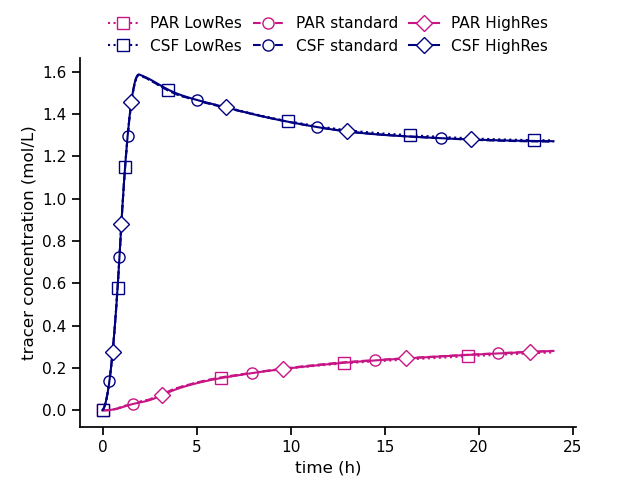
\includegraphics[width = 1 \linewidth]{figures/mesh_refinement_par_csf_mean.png}
        \caption{Mean tracer concentration in CSF and parenchyma under mesh refinement}
    \end{subfigure}
    \begin{subfigure}[b]{0.45\textwidth}
        \centering
     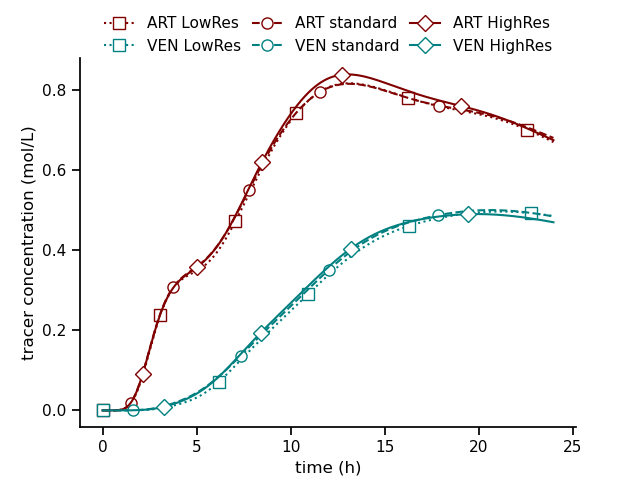
\includegraphics[width= 1 \linewidth]{figures/mesh_refinement_art_ven_mean.png}
         \caption{Mean tracer concentration in PVSs around (veins and) arteries  under mesh refinement}
    \end{subfigure}
    \caption{Mean tracer concentrations over the first 24\,h after injection on the CSF and parenchyma (a), and the arterial and venous PVS (b) computed on the LowRes, standard and HighRes meshes with a timestep of $dt=120$\,s.}
    \label{fig:mesh_convergence_concentrations}
\end{figure}


\begin{figure}
    \centering
    \begin{subfigure}[b]{0.49\textwidth}
        \centering
        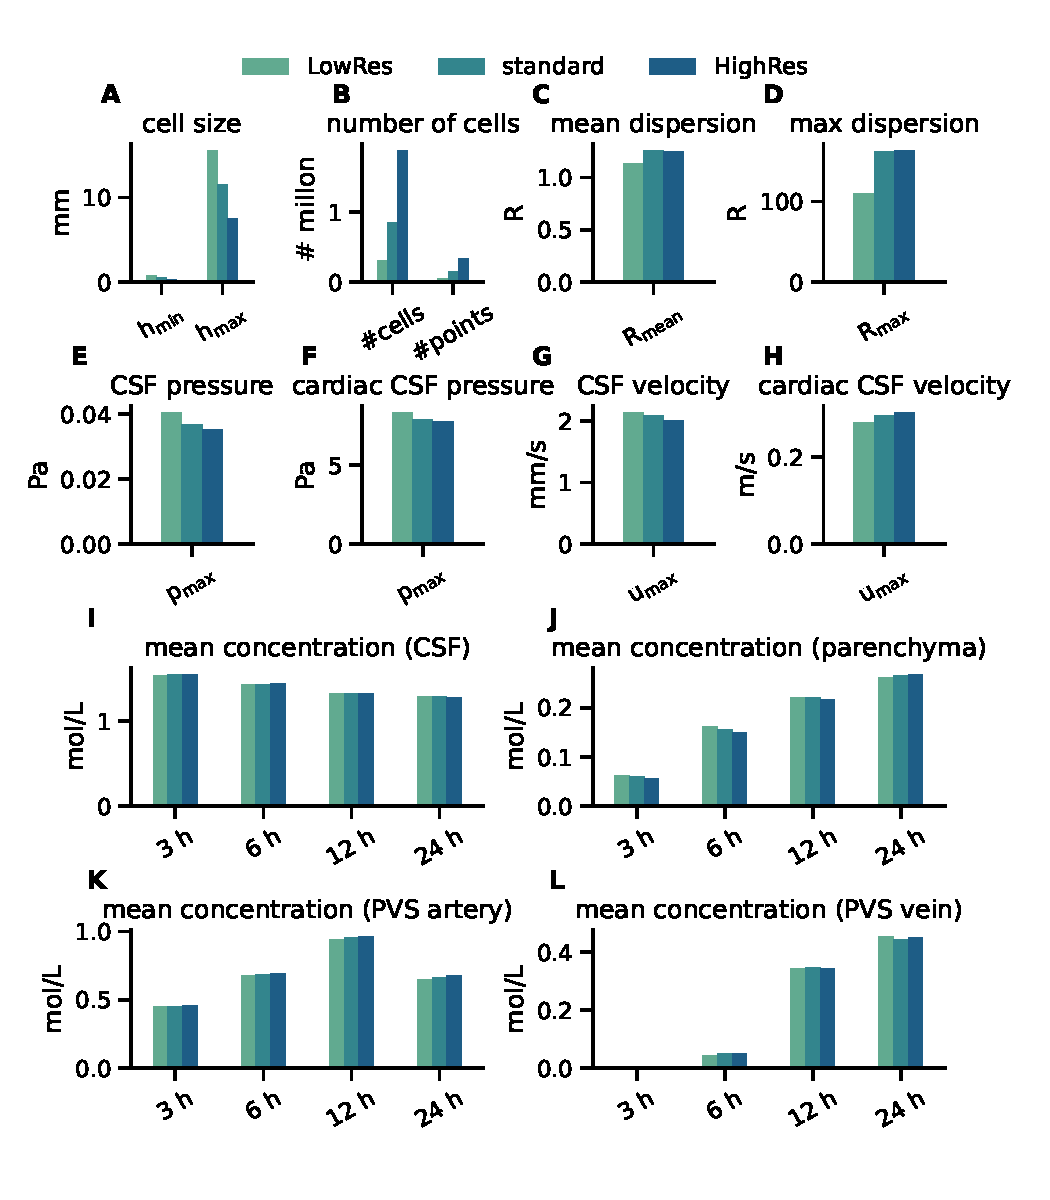
\includegraphics[trim={0.5cm 1cm 0.05cm 0.8cm}, clip, width = 1.05 \linewidth]{figures/mesh_refinement.pdf}
        \caption{Convergence of key quantities of interest with mesh refinement}
        \label{fig:mesh_convergence}
    \end{subfigure}
    \begin{subfigure}[b]{0.49\textwidth}
        \centering
     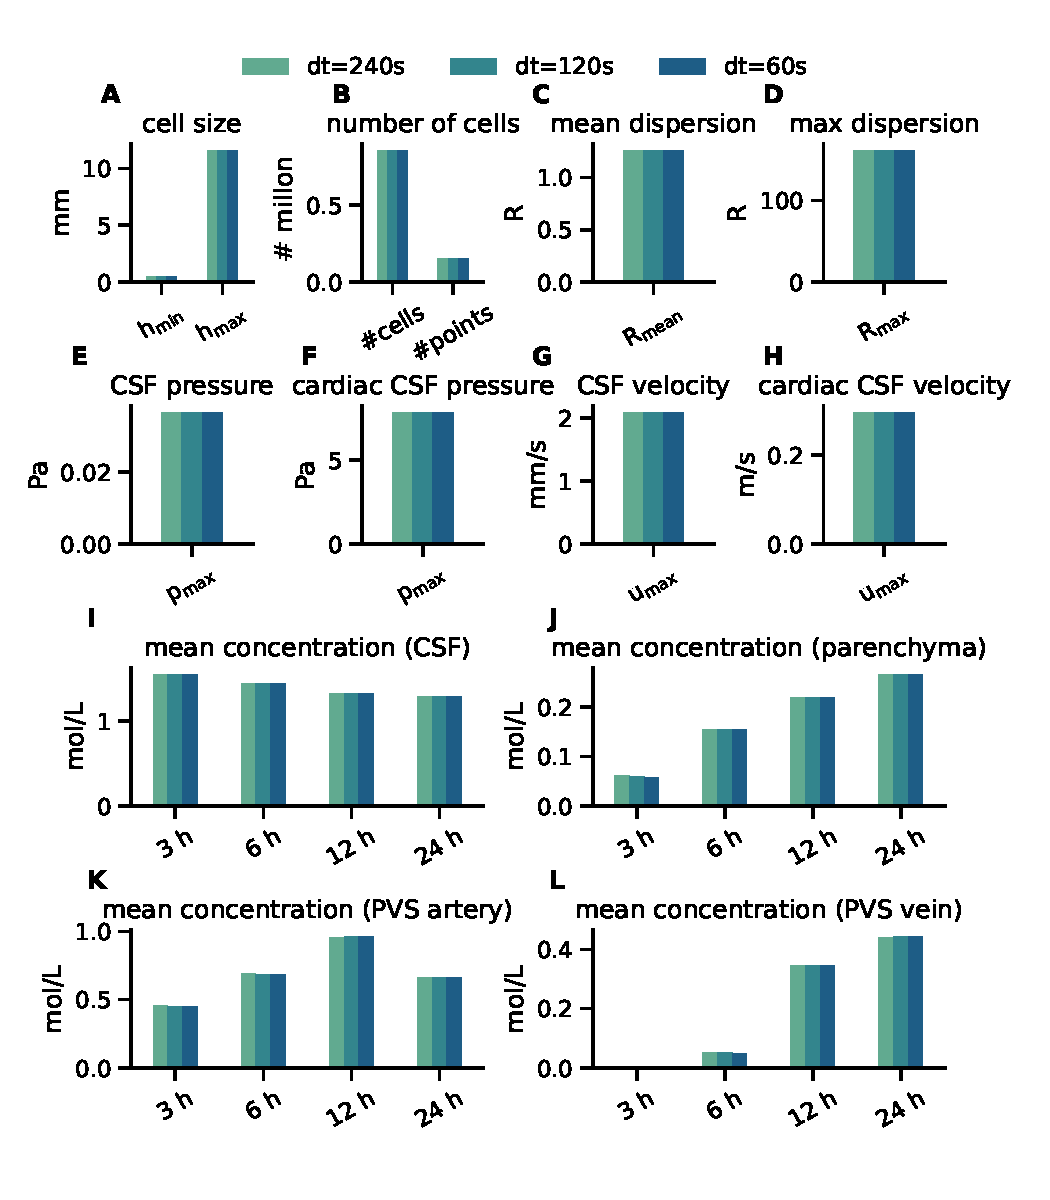
\includegraphics[trim={0.5cm 1cm 0.05cm 0.8cm}, clip,width= 1.05 \linewidth]{figures/time_refinement.pdf}
        \caption{Convergence of key quantities of interest with time refinement}
        \label{fig:time_convergence}
    \end{subfigure}
    \caption{minimal ($\rm h_{min}$) and maximal ($\rm h_{max}$) mesh cell sizes (computed as cell circumradius $\times 2$) (A); number of points and tetrahedral cells in each mesh (B); mean dispersion enhancement factor $R$ (C), maximum dispersion enhancement factor $R$ (D); maximum pressure in steady CSF production flow (E), maximum pressure in cardiac-driven CSF flow (F); maximum CSF velocity in steady CSF production flow (G); maximum CSF velocity in cardiac-driven CSF flow (H);  mean tracer concentration in the CSF, parenchyma, arterial PVS and venous PVS at 3,6,12 and 24\,h (I, J, K and L).}
\end{figure}

\begin{figure}
    \centering
    \begin{subfigure}[b]{0.45\textwidth}
        \centering
        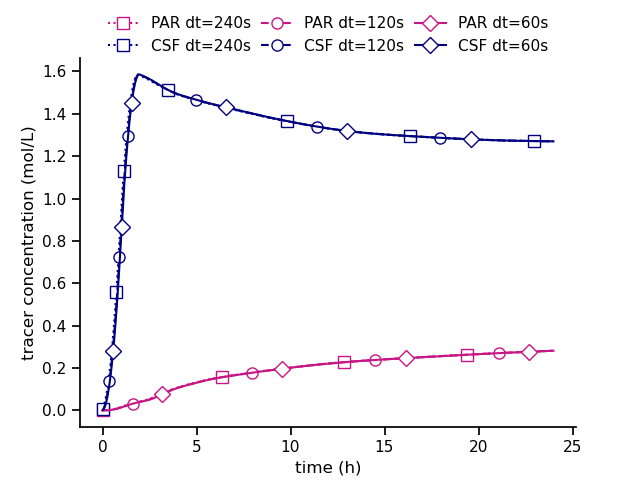
\includegraphics[width = 1 \linewidth]{figures/time_refinement_par_csf_mean.png}
        \caption{Mean tracer concentration in CSF and parenchyma under time step refinement}
    \end{subfigure}
    \begin{subfigure}[b]{0.45\textwidth}
        \centering
     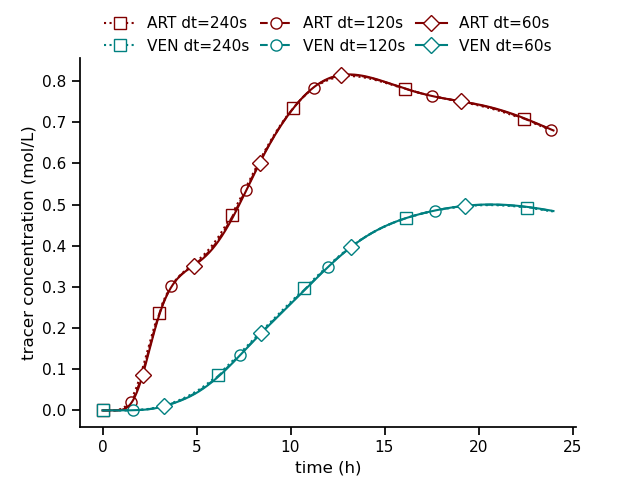
\includegraphics[width= 1\linewidth]{figures/time_refinement_art_ven_mean.png}
         \caption{Mean tracer concentration in PVSs around (veins and) arteries under time step refinement}
    \end{subfigure}
    \caption{Mean tracer concentrations over the first 24\,h after injection on the CSF and parenchyma (a), and the arterial and venous PVS (b) computed on the standard resolution mesh for timesteps $dt \in \{60, 120, 240 \}$\,s.}    \label{fig:time_convergence_concentrations}
\end{figure}


\newpage
\section{Notes}

Various notes associated with \cite{eide2024functional}:
\begin{itemize}
  \item
    Can observations of tracer indicate compartmentalization without
    the existence of physical barriers but in the presence of
    e.g.~substantial flow? We made observations in this direction in
    \cite{vinje2021brain}, relating to the then-active
    shape-of-perivascular-spaces discussion. We can address this by
    trying to quantify and evaluate the permeability of the PVS-SAS
    interface - comparing model predictions with the timings and
    patterns presented by \cite{eide2024functional}.
  \item
    Do the tracer primarily move from the PVS into the SAS or along
    (more slowly) along the SAS? This is left as an open question by
    \cite{eide2024functional} (page 3)
  \item
    How do altered ICP affect transport? Note that PVSAS transport is
    impaired (delayed) with increasing mean wave amplitude in the ICP
    signal and for iNPH patients (with enlarged PVSAS spaces).
  \item
    Very useful reference for PVS sizes (10--20 mm$^2$ in reference
    patients, 15-70 mm$^2$ in iNPH), and average propagation speeds.
\end{itemize}
